\documentclass[12pt]{article}
\usepackage[utf8x]{inputenc}
\usepackage{amsmath}
\usepackage{amsfonts}
\usepackage{mathrsfs}
\usepackage{natbib}
\usepackage{graphicx} % figuras
\usepackage[export]{adjustbox} % loads also graphicx
\usepackage{float}
\usepackage[font=footnotesize]{caption}
\usepackage{wrapfig}
\usepackage{authblk}
\usepackage{subfigure}
\usepackage{pifont}
\usepackage{a4wide}
%\usepackage{lipsum}
\topmargin=-2pt
\title{Name?}

\author[1]{G. B. Diaz Cortes}  
\author[1]{C. Vuik} 
\author[2]{J. D. Jansen} 
\affil[1]{Department of Applied Mathematics, TU Delft}
\affil[2]{Department of Geoscience \& Engineering, TU Delft}
\renewcommand\Authands{ and }
\date{March 2016}
\begin{document}



% Title Page

\newpage
\subsection*{Compressible Problem}

\begin{wrapfigure}{R}{5cm}
\centering 
\vspace{-10pt}
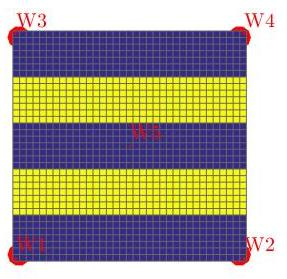
\includegraphics[width=4.5cm,height=4.5cm,keepaspectratio]{perm_comp.jpg}
 \vspace{-5pt}
\caption{ Heterogeneous permeability, 5 wells, compressible problem.}\label{fig:pc}
\vspace{-15pt}
\end{wrapfigure} 

A grid of $35\times 35$ cells is used with Neumann boundary conditions only. The domain consists of layers with two different permeability values (see Figure \ref{fig:pc}). The first layer has a permeability of $\sigma_1 = 30mD$, and the permeability of the second layer is $\sigma_2 = 3mD$. Therefore the permeability contrast between the layers is $10^{-1}$.The initial pressure of the reservoir is set as 200 bars. Four wells are positioned in the corners of the domain with a bhp of 100 bars, and a well is placed in the center of the domain with a bhp of 600 bars.
 For the first set of problems, we use the updated solution of the first 10 time steps with the same configuration as the problem as deflation vectors. We solve the rest of the time steps with DICCG$_{10}$ method with the 10 snapshots as deflation vectors and with 5 basis POD vectors as deflation vectors, DICCG$_{POD}$.
 For the second set of experiments, we use the same configuration as in the original problem but we vary the configuration of the wells. One corner well has the same pressure as the reservoir (200 bar), the other corner wells have a pressure of 100 bars and the central well has a pressure of 500 bars. 

\begin{itemize}
\begin{minipage}{.6\textwidth}
\item[]  $System$ $configuration$
\item[] Initial pressure 200 bar.
 \item[]  W1 =  W2 = W3 = W4 = 100 bar.
 \item[] W5 = 600 bars.\\
 \end{minipage}%
\begin{minipage}{.4\textwidth}
\item[] $Boundary$ $conditions:$\\
\item[] $\frac{\partial P(y=1)}{\partial n}=\frac{\partial P(y=ny)}{\partial n}=$
\item[] $\frac{\partial P(x=1)}{\partial n}=\frac{\partial P(x=nx)}{\partial n}=0$.
\end{minipage}
\begin{minipage}{.8\textwidth}
\item[] \emph{Snapshots (second set of experiments)}
 \item[] $\mathbf{z}_1$:  W2 = W3 = W4 =  100 bars, 
 W1 = 200 bars, W5 = 500 bars.
\item[] $\mathbf{z}_2$: W1 = W3 = W4 = 100 bars,
 W2 = 200 bars, W5 = 500 bars.
\item[] $\mathbf{z}_3$: W1 = W2 = W4 = 100 bars,
 W3 = 200 bars, W5 =  500 bars.
\item[] $\mathbf{z}_4$:  W1 = W2 = W3 = 100 bars,
 W4 = 200 bars, W5 =  500 bars.\\
\end{minipage}%
\end{itemize}
The simulation was performed during 152 days with 52 time steps and a time step of 3 days. The tolerance of the NR method and the linear solvers is $10^{-5}$.\\
\emph{\textbf{Case 1}}\\
In Figure \ref{fig:compsol}, the solution obtained with the ICCG method is presented, the solution is the same for all methods. The upper left figure represents the pressure field at the final time step. The upper right figure represents the pressure across the diagonal joining the (0,0) and (35,35) grid cells for all the timesteps. We observe the initial pressure (200 bars) in this diagonal and the evolution of the pressure field through time. In the lower figure we observe the surface volume rate for the five wells during the simulation.\\

\newpage
\section{Accuracy NR iteration $10^{-4}$}
%The eigenvalues of the covariance matrix  $\bar{\mathbf{R}}=\frac{1}{m}\sum_{i=1}^{m}(\mathbf{z}_i-\mathbf{z})(\mathbf{z}_i-\mathbf{z})^T$ are presented in Figure \ref{fig:eig_PODr}.\\

\begin{figure}[!h]
\centering
\begin{minipage}{.4\textwidth}
 \centering
\includegraphics[width=8cm,height=8cm,keepaspectratio]
{/home/wagm/cortes/Localdisk/Results/16_09/08/size_35perm_1_5wells_c_1e-3_s_52NR_4/iterations_4NR.jpg}
\caption{Number of iterations of the ICCG method for the first four NR iterations, accuracy NR iteration $10^{-4}$.}
\label{fig:NR_IC_4}
\end{minipage}%
\hspace{15mm}
\begin{minipage}{.4\textwidth}
 \centering
 \vspace{-5mm}
\includegraphics[width=8.5cm,height=8.5cm,keepaspectratio]
{/home/wagm/cortes/Localdisk/Results/16_09/08/size_35perm_1_5wells_c_1e-3_s_52NR_4/error_NR_zoom.jpg}
\caption{Error of the NR iteration for each timestep, accuracy NR iteration $10^{-4}$.}
\label{fig:error_NR_4}
\end{minipage}
\end{figure}



\begin{figure}[!h]
\centering
\begin{minipage}{.4\textwidth}
 \centering
\includegraphics[width=8cm,height=8cm,keepaspectratio]
{/home/wagm/cortes/Localdisk/Results/16_09/08/size_35perm_1_5wells_c_1e-3_s_52NR_4dv_10/iterations_4NR.jpg}
\caption{Number of iterations of the DICCG method for the first four NR iterations, accuracy NR iteration $10^{-4}$.}
\label{fig:NR_IC_4}
\end{minipage}%
\hspace{15mm}
\begin{minipage}{.4\textwidth}
 \centering
 \vspace{-5mm}
\includegraphics[width=8.5cm,height=8.5cm,keepaspectratio]
{/home/wagm/cortes/Localdisk/Results/16_09/08/size_35perm_1_5wells_c_1e-3_s_52NR_4dv_10/error_NR_zoom.jpg}
\caption{Error of the NR iteration for each timestep, accuracy NR iteration $10^{-4}$.}
\label{fig:error_NR_4}
\end{minipage}
\end{figure}



\newpage
\section{Accuracy NR iteration $10^{-5}$}
%The eigenvalues of the covariance matrix  $\bar{\mathbf{R}}=\frac{1}{m}\sum_{i=1}^{m}(\mathbf{z}_i-\mathbf{z})(\mathbf{z}_i-\mathbf{z})^T$ are presented in Figure \ref{fig:eig_PODr}.\\

\begin{figure}[!h]
\centering
\begin{minipage}{.4\textwidth}
 \centering
\includegraphics[width=8cm,height=8cm,keepaspectratio]
{/home/wagm/cortes/Localdisk/Results/16_09/08/size_35perm_1_5wells_c_1e-3_s_52NR_5/iterations_4NR.jpg}
\caption{Number of iterations of the ICCG method for the first four NR iterations, accuracy NR iteration $10^{-5}$.}
\label{fig:NR_IC_5}
\end{minipage}%
\hspace{15mm}
\begin{minipage}{.4\textwidth}
 \centering
 \vspace{-5mm}
\includegraphics[width=8.5cm,height=8.5cm,keepaspectratio]
{/home/wagm/cortes/Localdisk/Results/16_09/08/size_35perm_1_5wells_c_1e-3_s_52NR_5/error_NR_zoom.jpg}
\caption{Error of the NR iteration for each timestep, accuracy NR iteration $10^{-5}$.}
\label{fig:error_NR_5}
\end{minipage}
\end{figure}



\begin{figure}[!h]
\centering
\begin{minipage}{.4\textwidth}
 \centering
\includegraphics[width=8cm,height=8cm,keepaspectratio]
{/home/wagm/cortes/Localdisk/Results/16_09/08/size_35perm_1_5wells_c_1e-3_s_52NR_5dv_10/iterations_4NR.jpg}
\caption{Number of iterations of the DICCG method for the first four NR iterations, accuracy NR iteration $10^{-4}$.}
\label{fig:NR_IC_4}
\end{minipage}%
\hspace{15mm}
\begin{minipage}{.4\textwidth}
 \centering
 \vspace{-5mm}
\includegraphics[width=8.5cm,height=8.5cm,keepaspectratio]
{/home/wagm/cortes/Localdisk/Results/16_09/08/size_35perm_1_5wells_c_1e-3_s_52NR_5dv_10/error_NR_zoom.jpg}
\caption{Error of the NR iteration for each timestep, accuracy NR iteration $10^{-4}$.}
\label{fig:error_NR_4}
\end{minipage}
\end{figure}



\newpage
\section{Accuracy NR iteration $10^{-6}$}
\begin{figure}[!h]
\centering
\begin{minipage}{.4\textwidth}
 \centering
\includegraphics[width=8cm,height=8cm,keepaspectratio]
{/home/wagm/cortes/Localdisk/Results/16_09/08/size_35perm_1_5wells_c_1e-3_s_52NR_6/iterations_4NR.jpg}
\caption{Number of iterations of the ICCG method for the first four NR iterations, accuracy NR iteration $10^{-6}$.}
\label{fig:NR_IC_6}
\end{minipage}%
\hspace{15mm}
\begin{minipage}{.4\textwidth}
 \centering
 \vspace{-5mm}
\includegraphics[width=8.5cm,height=8.5cm,keepaspectratio]
{/home/wagm/cortes/Localdisk/Results/16_09/08/size_35perm_1_5wells_c_1e-3_s_52NR_6/error_NR_zoom.jpg}
\caption{Error of the NR iteration for each timestep, accuracy NR iteration $10^{-6}$.}
\label{fig:error_NR_6}
\end{minipage}
\end{figure}



\begin{figure}[!h]
\centering
\begin{minipage}{.4\textwidth}
 \centering
\includegraphics[width=8cm,height=8cm,keepaspectratio]
{/home/wagm/cortes/Localdisk/Results/16_09/08/size_35perm_1_5wells_c_1e-3_s_52NR_6dv_10/iterations_4NR.jpg}
\caption{Number of iterations of the DICCG method for the first four NR iterations, accuracy NR iteration $10^{-6}$.}
\label{fig:NR_IC_6}
\end{minipage}%
\hspace{15mm}
\begin{minipage}{.4\textwidth}
 \centering
 \vspace{-5mm}
\includegraphics[width=8.5cm,height=8.5cm,keepaspectratio]
{/home/wagm/cortes/Localdisk/Results/16_09/08/size_35perm_1_5wells_c_1e-3_s_52NR_6dv_10/error_NR_zoom.jpg}
\caption{Error of the NR iteration for each timestep, accuracy NR iteration $10^{-6}$.}
\label{fig:error_NR_6}
\end{minipage}
\end{figure}

\newpage
\section{Accuracy NR iteration $10^{-7}$}
\begin{figure}[!h]
\centering
\begin{minipage}{.4\textwidth}
 \centering
\includegraphics[width=8cm,height=8cm,keepaspectratio]
{/home/wagm/cortes/Localdisk/Results/16_09/08/size_35perm_1_5wells_c_1e-3_s_52NR_7/iterations_4NR.jpg}
\caption{Number of iterations of the ICCG method for the first four NR iterations, accuracy NR iteration $10^{-7}$.}
\label{fig:NR_IC_7}
\end{minipage}%
\hspace{15mm}
\begin{minipage}{.4\textwidth}
 \centering
 \vspace{-5mm}
\includegraphics[width=8.5cm,height=8.5cm,keepaspectratio]
{/home/wagm/cortes/Localdisk/Results/16_09/08/size_35perm_1_5wells_c_1e-3_s_52NR_7/error_NR_zoom.jpg}
\caption{Error of the NR iteration for each timestep, accuracy NR iteration $10^{-7}$.}
\label{fig:error_NR_7}
\end{minipage}
\end{figure}



\begin{figure}[!h]
\centering
\begin{minipage}{.4\textwidth}
 \centering
\includegraphics[width=8cm,height=8cm,keepaspectratio]
{/home/wagm/cortes/Localdisk/Results/16_09/08/size_35perm_1_5wells_c_1e-3_s_52NR_7dv_10/iterations_4NR.jpg}
\caption{Number of iterations of the DICCG method for the first four NR iterations, accuracy NR iteration $10^{-7}$.}
\label{fig:NR_IC_7}
\end{minipage}%
\hspace{15mm}
\begin{minipage}{.4\textwidth}
 \centering
 \vspace{-5mm}
\includegraphics[width=8.5cm,height=8.5cm,keepaspectratio]
{/home/wagm/cortes/Localdisk/Results/16_09/08/size_35perm_1_5wells_c_1e-3_s_52NR_7dv_10/error_NR_zoom.jpg}
\caption{Error of the NR iteration for each timestep, accuracy NR iteration $10^{-7}$.}
\label{fig:error_NR_7}
\end{minipage}
\end{figure}


\newpage
\section{Size 35 x 35}
\begin{figure}[!h]
\centering
\begin{minipage}{.4\textwidth}
 \centering
\includegraphics[width=8cm,height=8cm,keepaspectratio]
{/home/wagm/cortes/Localdisk/Results/16_09/08/size_35perm_1_5wells_c_1e-3_s_52NR_5/iterations_4NR.jpg}
\caption{Number of iterations of the ICCG method for the first four NR iterations, size 35 x 35.}
\label{fig:NR_IC_35}
\end{minipage}%
\hspace{15mm}
\begin{minipage}{.4\textwidth}
 \centering
 \vspace{-5mm}
\includegraphics[width=8.5cm,height=8.5cm,keepaspectratio]
{/home/wagm/cortes/Localdisk/Results/16_09/08/size_35perm_1_5wells_c_1e-3_s_52NR_5/error_NR_zoom.jpg}
\caption{Error of the NR iteration for each timestep, size 35 x 35.}
\label{fig:error_NR_35}
\end{minipage}
\end{figure}



\begin{figure}[!h]
\centering
\begin{minipage}{.4\textwidth}
 \centering
\includegraphics[width=8cm,height=8cm,keepaspectratio]
{/home/wagm/cortes/Localdisk/Results/16_09/08/size_35perm_1_5wells_c_1e-3_s_52NR_5dv_10/iterations_4NR.jpg}
\caption{Number of iterations of the DICCG method for the first four NR iterations, size 35 x 35.}
\label{fig:NR_IC_35}
\end{minipage}%
\hspace{15mm}
\begin{minipage}{.4\textwidth}
 \centering
 \vspace{-5mm}
\includegraphics[width=8.5cm,height=8.5cm,keepaspectratio]
{/home/wagm/cortes/Localdisk/Results/16_09/08/size_35perm_1_5wells_c_1e-3_s_52NR_5dv_10/error_NR_zoom.jpg}
\caption{Error of the NR iteration for each timestep, size 35 x 35.}
\label{fig:error_NR_35}
\end{minipage}
\end{figure}

\newpage
\section{Size 70 x 70}
\begin{figure}[!h]
\centering
\begin{minipage}{.4\textwidth}
 \centering
\includegraphics[width=8cm,height=8cm,keepaspectratio]
{/home/wagm/cortes/Localdisk/Results/16_09/09/size_70perm_1_5wells_c_1e-3_s_52/iterations_4NR.jpg}
\caption{Number of iterations of the ICCG method for the first four NR iterations, size 70 x 70.}
\label{fig:NR_IC_70}
\end{minipage}%
\hspace{15mm}
\begin{minipage}{.4\textwidth}
 \centering
 \vspace{-5mm}
\includegraphics[width=8.5cm,height=8.5cm,keepaspectratio]
{/home/wagm/cortes/Localdisk/Results/16_09/09/size_70perm_1_5wells_c_1e-3_s_52/error_NR_zoom.jpg}
\caption{Error of the NR iteration for each timestep, size 70 x 70.}
\label{fig:error_NR_70}
\end{minipage}
\end{figure}



\begin{figure}[!h]
\centering
\begin{minipage}{.4\textwidth}
 \centering
\includegraphics[width=8cm,height=8cm,keepaspectratio]
{/home/wagm/cortes/Localdisk/Results/16_09/09/size_70perm_1_5wells_c_1e-3_s_52dv_10/iterations_4NR.jpg}
\caption{Number of iterations of the DICCG method for the first four NR iterations, size 70 x 70.}
\label{fig:NR_IC_70}
\end{minipage}%
\hspace{15mm}
\begin{minipage}{.4\textwidth}
 \centering
 \vspace{-5mm}
\includegraphics[width=8.5cm,height=8.5cm,keepaspectratio]
{/home/wagm/cortes/Localdisk/Results/16_09/09/size_70perm_1_5wells_c_1e-3_s_52dv_10/error_NR_zoom.jpg}
\caption{Error of the NR iteration for each timestep, size 70 x 70.}
\label{fig:error_NR_70}
\end{minipage}
\end{figure}

\newpage
\section{Size 70 x 70}
\begin{figure}[!h]
\centering
\begin{minipage}{.4\textwidth}
 \centering
\includegraphics[width=8cm,height=8cm,keepaspectratio]
{/home/wagm/cortes/Localdisk/Results/16_09/09/size_70perm_1_5wells_c_1e-3_s_52/iterations_4NR.jpg}
\caption{Number of iterations of the ICCG method for the first four NR iterations, size 70 x 70.}
\label{fig:NR_IC_70}
\end{minipage}%
\hspace{15mm}
\begin{minipage}{.4\textwidth}
 \centering
 \vspace{-5mm}
\includegraphics[width=8.5cm,height=8.5cm,keepaspectratio]
{/home/wagm/cortes/Localdisk/Results/16_09/09/size_70perm_1_5wells_c_1e-3_s_52/error_NR_zoom.jpg}
\caption{Error of the NR iteration for each timestep, size 70 x 70.}
\label{fig:error_NR_70}
\end{minipage}
\end{figure}



\begin{figure}[!h]
\centering
\begin{minipage}{.4\textwidth}
 \centering
\includegraphics[width=8cm,height=8cm,keepaspectratio]
{/home/wagm/cortes/Localdisk/Results/16_09/09/size_70perm_1_5wells_c_1e-3_s_52dv_15/iterations_4NR.jpg}
\caption{Number of iterations of the DICCG method for the first four NR iterations, size 70 x 70, 15 deflation vectors.}
\label{fig:NR_IC_70}
\end{minipage}%
\hspace{15mm}
\begin{minipage}{.4\textwidth}
 \centering
 \vspace{-5mm}
\includegraphics[width=8.5cm,height=8.5cm,keepaspectratio]
{/home/wagm/cortes/Localdisk/Results/16_09/09/size_70perm_1_5wells_c_1e-3_s_52dv_15/error_NR_zoom.jpg}
\caption{Error of the NR iteration for each timestep, size 70 x 70, 15 deflation vectors.}
\label{fig:error_NR_70}
\end{minipage}
\end{figure}



\newpage
\section{Size 105 x 105}
\begin{figure}[!h]
\centering
\begin{minipage}{.4\textwidth}
 \centering
\includegraphics[width=8cm,height=8cm,keepaspectratio]
{/home/wagm/cortes/Localdisk/Results/16_09/09/size_105perm_1_5wells_c_1e-3_s_52/iterations_4NR.jpg}
\caption{Number of iterations of the ICCG method for the first four NR iterations, size 105 x 105.}
\label{fig:NR_IC_105}
\end{minipage}%
\hspace{15mm}
\begin{minipage}{.4\textwidth}
 \centering
 \vspace{-5mm}
\includegraphics[width=8.5cm,height=8.5cm,keepaspectratio]
{/home/wagm/cortes/Localdisk/Results/16_09/09/size_105perm_1_5wells_c_1e-3_s_52/error_NR_zoom.jpg}
\caption{Error of the NR iteration for each timestep, size 105 x 105.}
\label{fig:error_NR_105}
\end{minipage}
\end{figure}



\begin{figure}[!h]
\centering
\begin{minipage}{.4\textwidth}
 \centering
\includegraphics[width=8cm,height=8cm,keepaspectratio]
{/home/wagm/cortes/Localdisk/Results/16_09/09/size_105perm_1_5wells_c_1e-3_s_52dv_10/iterations_4NR.jpg}
\caption{Number of iterations of the DICCG method for the first four NR iterations, size 105 x 105.}
\label{fig:NR_IC_105}
\end{minipage}%
\hspace{15mm}
\begin{minipage}{.4\textwidth}
 \centering
 \vspace{-5mm}
\includegraphics[width=8.5cm,height=8.5cm,keepaspectratio]
{/home/wagm/cortes/Localdisk/Results/16_09/09/size_105perm_1_5wells_c_1e-3_s_52dv_10/error_NR_zoom.jpg}
\caption{Error of the NR iteration for each timestep, size 105 x 105.}
\label{fig:error_NR_105}
\end{minipage}
\end{figure}

\newpage
\section{Size 105 x 105}
\begin{figure}[!h]
\centering
\begin{minipage}{.4\textwidth}
 \centering
\includegraphics[width=8cm,height=8cm,keepaspectratio]
{/home/wagm/cortes/Localdisk/Results/16_09/09/size_105perm_1_5wells_c_1e-3_s_52/iterations_4NR.jpg}
\caption{Number of iterations of the ICCG method for the first four NR iterations, size 105 x 105.}
\label{fig:NR_IC_105}
\end{minipage}%
\hspace{15mm}
\begin{minipage}{.4\textwidth}
 \centering
 \vspace{-5mm}
\includegraphics[width=8.5cm,height=8.5cm,keepaspectratio]
{/home/wagm/cortes/Localdisk/Results/16_09/09/size_105perm_1_5wells_c_1e-3_s_52/error_NR_zoom.jpg}
\caption{Error of the NR iteration for each timestep, size 105 x 105.}
\label{fig:error_NR_105}
\end{minipage}
\end{figure}



\begin{figure}[!h]
\centering
\begin{minipage}{.4\textwidth}
 \centering
\includegraphics[width=8cm,height=8cm,keepaspectratio]
{/home/wagm/cortes/Localdisk/Results/16_09/09/size_105perm_1_5wells_c_1e-3_s_52dv_15/iterations_4NR.jpg}
\caption{Number of iterations of the DICCG method for the first four NR iterations, size 105 x 105, 15 deflation vectors.}
\label{fig:NR_IC_105}
\end{minipage}%
\hspace{15mm}
\begin{minipage}{.4\textwidth}
 \centering
 \vspace{-5mm}
\includegraphics[width=8.5cm,height=8.5cm,keepaspectratio]
{/home/wagm/cortes/Localdisk/Results/16_09/09/size_105perm_1_5wells_c_1e-3_s_52dv_15/error_NR_zoom.jpg}
\caption{Error of the NR iteration for each timestep, size 105 x 105, 15 deflation vectors.}
\label{fig:error_NR_105}
\end{minipage}
\end{figure}

\newpage
\section{Size 105 x 105}
\begin{figure}[!h]
\centering
\begin{minipage}{.4\textwidth}
 \centering
\includegraphics[width=8cm,height=8cm,keepaspectratio]
{/home/wagm/cortes/Localdisk/Results/16_09/09/size_105perm_1_5wells_c_1e-3_s_52/iterations_4NR.jpg}
\caption{Number of iterations of the ICCG method for the first four NR iterations, size 105 x 105.}
\label{fig:NR_IC_105}
\end{minipage}%
\hspace{15mm}
\begin{minipage}{.4\textwidth}
 \centering
 \vspace{-5mm}
\includegraphics[width=8.5cm,height=8.5cm,keepaspectratio]
{/home/wagm/cortes/Localdisk/Results/16_09/09/size_105perm_1_5wells_c_1e-3_s_52/error_NR_zoom.jpg}
\caption{Error of the NR iteration for each timestep, size 105 x 105.}
\label{fig:error_NR_105}
\end{minipage}
\end{figure}



\begin{figure}[!h]
\centering
\begin{minipage}{.4\textwidth}
 \centering
\includegraphics[width=8cm,height=8cm,keepaspectratio]
{/home/wagm/cortes/Localdisk/Results/16_09/09/size_105perm_1_5wells_c_1e-3_s_52dv_25pod10-25/iterations_4NR.jpg}
\caption{Number of iterations of the DICCG method for the first four NR iterations, size 105 x 105, 25 deflation vectors, POD (10-25).}
\label{fig:NR_IC_105}
\end{minipage}%
\hspace{15mm}
\begin{minipage}{.4\textwidth}
 \centering
 \vspace{-5mm}
\includegraphics[width=8.5cm,height=8.5cm,keepaspectratio]
{/home/wagm/cortes/Localdisk/Results/16_09/09/size_105perm_1_5wells_c_1e-3_s_52dv_25pod10-25/error_NR_zoom.jpg}
\caption{Error of the NR iteration for each timestep, size 105 x 105, 25 deflation vectors, POD (10-25).}
\label{fig:error_NR_105}
\end{minipage}
\end{figure}


\newpage
\section{Contrast in permeability $10^{-1}$}
\begin{figure}[!h]
\centering
\begin{minipage}{.4\textwidth}
 \centering
\includegraphics[width=8cm,height=8cm,keepaspectratio]
{/home/wagm/cortes/Localdisk/Results/16_09/12/size_35perm_1_5wells_c_1e-3_s_52/iterations_4NR.jpg}
\caption{Number of iterations of the ICCG method for the first four NR iterations, size 35 x 35, contrast in permeability $10^{-1}$.}
\label{fig:PER_IC_1}
\end{minipage}%
\hspace{15mm}
\begin{minipage}{.4\textwidth}
 \centering
 \vspace{-5mm}
\includegraphics[width=8.5cm,height=8.5cm,keepaspectratio]
{/home/wagm/cortes/Localdisk/Results/16_09/12/size_35perm_1_5wells_c_1e-3_s_52/error_NR_zoom.jpg}
\caption{Error of the NR iteration for each timestep, size 35 x 35, contrast in permeability $10^{-1}$.}
\label{fig:error_PER_IC_1}
\end{minipage}
\end{figure}



\begin{figure}[!h]
\centering
\begin{minipage}{.4\textwidth}
 \centering
\includegraphics[width=8cm,height=8cm,keepaspectratio]
{/home/wagm/cortes/Localdisk/Results/16_09/12/size_35perm_1_5wells_c_1e-3_s_52dv_10/iterations_4NR.jpg}
\caption{Number of iterations of the DICCG method for the first four NR iterations, size 35 x 35, contrast in permeability $10^{-1}$.}
\label{fig:PER_DIC_1}
\end{minipage}%
\hspace{15mm}
\begin{minipage}{.4\textwidth}
 \centering
 \vspace{-5mm}
\includegraphics[width=8.5cm,height=8.5cm,keepaspectratio]
{/home/wagm/cortes/Localdisk/Results/16_09/12/size_35perm_1_5wells_c_1e-3_s_52dv_10/error_NR_zoom.jpg}
\caption{Error of the NR iteration for each timestep, size 35 x 35, contrast in permeability $10^{-1}$.}
\label{fig:PER_DIC_1}
\end{minipage}
\end{figure}


\begin{figure}[!h]
\centering
\begin{minipage}{.4\textwidth}
 \centering
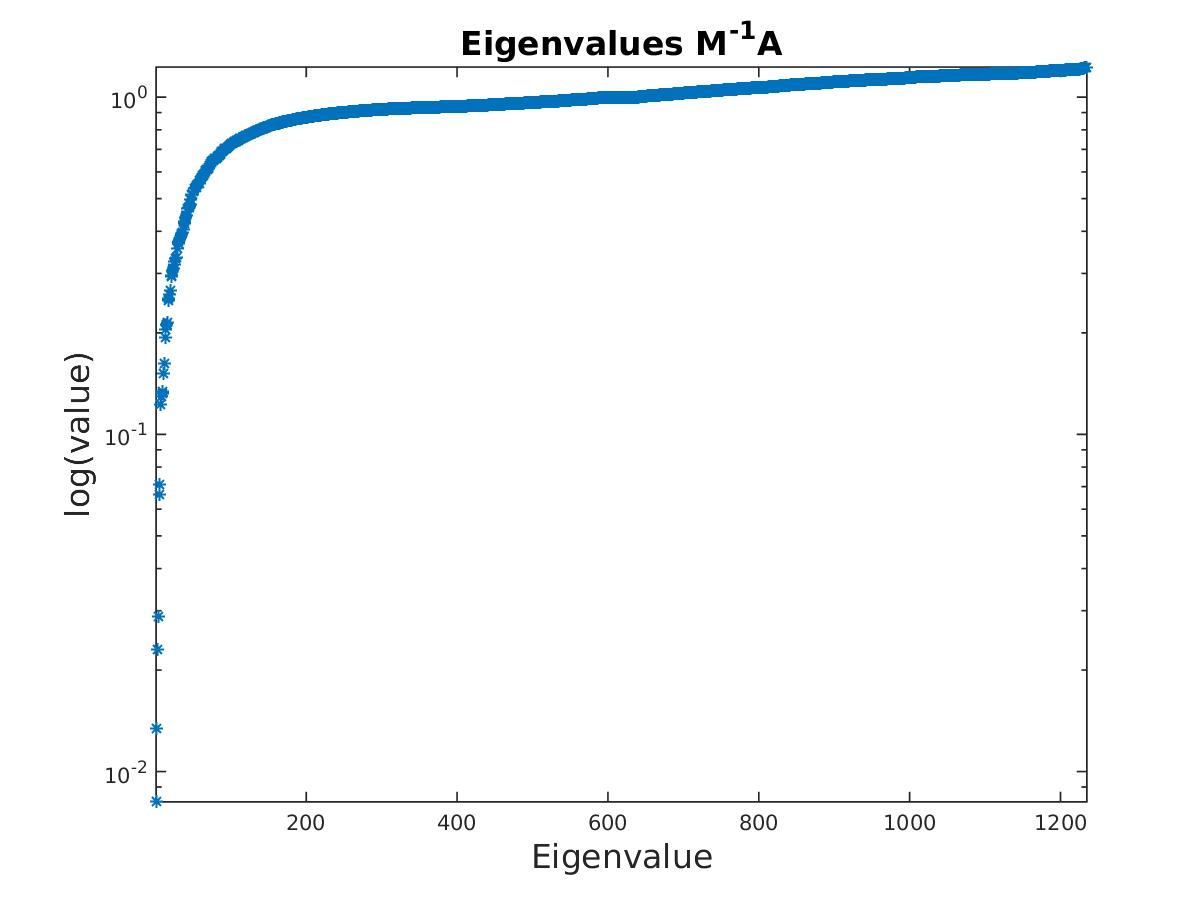
\includegraphics[width=7.5cm,height=7.5cm,keepaspectratio]
{/home/wagm/cortes/Localdisk/Results/16_09/12/size_35perm_1_5wells_c_1e-3_s_52/eigs/eigs1step.jpg}
\caption{Eigenvalues of the preconditioned system ICCG.}
\label{fig:eigs_PER_IC_1}
\end{minipage}%
\hspace{15mm}
\begin{minipage}{.4\textwidth}
 \centering
\includegraphics[width=7.5cm,height=7.5cm,keepaspectratio]
{/home/wagm/cortes/Localdisk/Results/16_09/12/size_35perm_1_5wells_c_1e-3_s_52dv_10/eigs/eigsPA11step.jpg}
\caption{Eigenvalues of the deflated system DICCG$_{10}$ with 10 deflation vectors.}
\label{fig:eigs_PER_DIC_1}
\end{minipage}
\end{figure}

\newpage
\section{Contrast in permeability $10^{-2}$}
\begin{figure}[!h]
\centering
\begin{minipage}{.4\textwidth}
 \centering
\includegraphics[width=8cm,height=8cm,keepaspectratio]
{/home/wagm/cortes/Localdisk/Results/16_09/12/size_35perm_2_5wells_c_1e-3_s_52/iterations_4NR.jpg}
\caption{Number of iterations of the ICCG method for the first four NR iterations, size 35 x 35, contrast in permeability $10^{-2}$.}
\label{fig:PER_IC_2}
\end{minipage}%
\hspace{15mm}
\begin{minipage}{.4\textwidth}
 \centering
 \vspace{-5mm}
\includegraphics[width=8.5cm,height=8.5cm,keepaspectratio]
{/home/wagm/cortes/Localdisk/Results/16_09/12/size_35perm_2_5wells_c_1e-3_s_52/error_NR_zoom.jpg}
\caption{Error of the NR iteration for each timestep, size 35 x 35, contrast in permeability $10^{-2}$.}
\label{fig:error_PER_IC_2}
\end{minipage}
\end{figure}


\subsection{10 deflation vectors}
\begin{figure}[!h]
\centering
\begin{minipage}{.4\textwidth}
 \centering
\includegraphics[width=8cm,height=8cm,keepaspectratio]
{/home/wagm/cortes/Localdisk/Results/16_09/12/size_35perm_2_5wells_c_1e-3_s_52dv_10/iterations_4NR.jpg}
\caption{Number of iterations of the DICCG method for the first four NR iterations, size 35 x 35, contrast in permeability $10^{-2}$.}
\label{fig:PER_DIC_2}
\end{minipage}%
\hspace{15mm}
\begin{minipage}{.4\textwidth}
 \centering
 \vspace{-5mm}
\includegraphics[width=8.5cm,height=8.5cm,keepaspectratio]
{/home/wagm/cortes/Localdisk/Results/16_09/12/size_35perm_2_5wells_c_1e-3_s_52dv_10/error_NR_zoom.jpg}
\caption{Error of the NR iteration for each timestep, size 35 x 35, contrast in permeability $10^{-2}$.}
\label{fig:PER_DIC_2}
\end{minipage}
\end{figure}


\begin{figure}[!h]
\centering
\begin{minipage}{.4\textwidth}
 \centering
\includegraphics[width=7.5cm,height=7.5cm,keepaspectratio]
{/home/wagm/cortes/Localdisk/Results/16_09/12/size_35perm_2_5wells_c_1e-3_s_52/eigs/eigs1step.jpg}
\caption{Eigenvalues of the preconditioned system ICCG.}
\label{fig:eigs_PER_IC_2}
\end{minipage}%
\hspace{15mm}
\begin{minipage}{.4\textwidth}
 \centering
\includegraphics[width=7.5cm,height=7.5cm,keepaspectratio]
{/home/wagm/cortes/Localdisk/Results/16_09/12/size_35perm_2_5wells_c_1e-3_s_52dv_10/eigs/eigsPA11step.jpg}
\caption{Eigenvalues of the deflated system DICCG$_{10}$ with 10 deflation vectors.}
\label{fig:eigs_PER_DIC_2}
\end{minipage}
\end{figure}
\newpage
\subsection{20 deflation vectors, 15 POD vectors}
\begin{figure}[!h]
\centering
\begin{minipage}{.4\textwidth}
 \centering
\includegraphics[width=8cm,height=8cm,keepaspectratio]
{/home/wagm/cortes/Localdisk/Results/16_09/12/size_35perm_2_5wells_c_1e-3_s_52dv_20pod6_20/iterations_4NR.jpg}
\caption{Number of iterations of the DICCG$_{POD15}$ method for the first four NR iterations, size 35 x 35, contrast in permeability $10^{-2}$.}
\label{fig:PER_DIC_2}
\end{minipage}%
\hspace{15mm}
\begin{minipage}{.4\textwidth}
 \centering
 \vspace{-5mm}
\includegraphics[width=8.5cm,height=8.5cm,keepaspectratio]
{/home/wagm/cortes/Localdisk/Results/16_09/12/size_35perm_2_5wells_c_1e-3_s_52dv_20pod6_20/error_NR_zoom.jpg}
\caption{Error of the NR iteration for each timestep, size 35 x 35, contrast in permeability $10^{-2}$.}
\label{fig:PER_DIC_2}
\end{minipage}
\end{figure}

\begin{figure}[!h]
\centering
\begin{minipage}{.4\textwidth}
 \centering
\includegraphics[width=7.5cm,height=7.5cm,keepaspectratio]
{/home/wagm/cortes/Localdisk/Results/16_09/12/size_35perm_2_5wells_c_1e-3_s_52/eigs/eigs1step.jpg}
\caption{Eigenvalues of the preconditioned system ICCG.}
\label{fig:eigs_PER_IC_2}
\end{minipage}%
\hspace{15mm}
\begin{minipage}{.4\textwidth}
 \centering
\includegraphics[width=7.5cm,height=7.5cm,keepaspectratio]
{/home/wagm/cortes/Localdisk/Results/16_09/12/size_35perm_2_5wells_c_1e-3_s_52dv_20pod6_20/eigs/eigsPA21step.jpg}
\caption{Eigenvalues of the deflated system DICCG$_{POD15}$ with 15 POD basis vectors obtained from 20 deflation vectors.}
\label{fig:eigs_PER_DIC_2}
\end{minipage}
\end{figure}


\newpage
\section{Contrast in permeability $10^{-3}$}
\begin{figure}[!h]
\centering
\begin{minipage}{.4\textwidth}
 \centering
\includegraphics[width=8cm,height=8cm,keepaspectratio]
{/home/wagm/cortes/Localdisk/Results/16_09/12/size_35perm_3_5wells_c_1e-3_s_52/iterations_4NR.jpg}
\caption{Number of iterations of the ICCG method for the first four NR iterations, size 35 x 35, contrast in permeability $10^{-3}$.}
\label{fig:PER_IC_3}
\end{minipage}%
\hspace{15mm}
\begin{minipage}{.4\textwidth}
 \centering
 \vspace{-5mm}
\includegraphics[width=8.5cm,height=8.5cm,keepaspectratio]
{/home/wagm/cortes/Localdisk/Results/16_09/12/size_35perm_3_5wells_c_1e-3_s_52/error_NR_zoom.jpg}
\caption{Error of the NR iteration for each timestep, size 35 x 35, contrast in permeability $10^{-3}$.}
\label{fig:error_PER_IC_3}
\end{minipage}
\end{figure}


\newpage
\subsection{20 deflation vectors, 15 POD vectors}
\begin{figure}[!h]
\centering
\begin{minipage}{.4\textwidth}
 \centering
\includegraphics[width=8cm,height=8cm,keepaspectratio]
{/home/wagm/cortes/Localdisk/Results/16_09/12/size_35perm_3_5wells_c_1e-3_s_52dv_20pod6_20/iterations_4NR.jpg}
\caption{Number of iterations of the DICCG$_{POD15}$ method for the first four NR iterations, size 35 x 35, contrast in permeability $10^{-3}$.}
\label{fig:PER_DIC_3}
\end{minipage}%
\hspace{15mm}
\begin{minipage}{.4\textwidth}
 \centering
 \vspace{-5mm}
\includegraphics[width=8.5cm,height=8.5cm,keepaspectratio]
{/home/wagm/cortes/Localdisk/Results/16_09/12/size_35perm_3_5wells_c_1e-3_s_52dv_20pod6_20/error_NR_zoom.jpg}
\caption{Error of the NR iteration for each timestep, size 35 x 35, contrast in permeability $10^{-3}$.}
\label{fig:PER_DIC_3}
\end{minipage}
\end{figure}

\begin{figure}[!h]
\centering
\begin{minipage}{.4\textwidth}
 \centering
\includegraphics[width=7.5cm,height=7.5cm,keepaspectratio]
{/home/wagm/cortes/Localdisk/Results/16_09/12/size_35perm_3_5wells_c_1e-3_s_52/eigs/eigs1step.jpg}
\caption{Eigenvalues of the preconditioned system ICCG.}
\label{fig:eigs_PER_IC_3}
\end{minipage}%
\hspace{15mm}
\begin{minipage}{.4\textwidth}
 \centering
\includegraphics[width=7.5cm,height=7.5cm,keepaspectratio]
{/home/wagm/cortes/Localdisk/Results/16_09/12/size_35perm_3_5wells_c_1e-3_s_52dv_20pod6_20/eigs/eigsPA21step.jpg}
\caption{Eigenvalues of the deflated system DICCG$_{POD15}$ with 15 POD basis vectors obtained from 20 deflation vectors.}
\label{fig:eigs_PER_DIC_3}
\end{minipage}
\end{figure}



\newpage
\subsection{30 deflation vectors, 25 POD vectors}
\begin{figure}[!h]
\centering
\begin{minipage}{.4\textwidth}
 \centering
\includegraphics[width=8cm,height=8cm,keepaspectratio]
{/home/wagm/cortes/Localdisk/Results/16_09/12/size_35perm_3_5wells_c_1e-3_s_52dv_30pod6_30/iterations_4NR.jpg}
\caption{Number of iterations of the DICCG$_{POD15}$ method for the first four NR iterations, size 35 x 35, contrast in permeability $10^{-3}$.}
\label{fig:PER_DIC_3}
\end{minipage}%
\hspace{15mm}
\begin{minipage}{.4\textwidth}
 \centering
 \vspace{-5mm}
\includegraphics[width=8.5cm,height=8.5cm,keepaspectratio]
{/home/wagm/cortes/Localdisk/Results/16_09/12/size_35perm_3_5wells_c_1e-3_s_52dv_30pod6_30/error_NR_zoom.jpg}
\caption{Error of the NR iteration for each timestep, size 35 x 35, contrast in permeability $10^{-3}$.}
\label{fig:PER_DIC_3}
\end{minipage}
\end{figure}

\begin{figure}[!h]
\centering
\begin{minipage}{.4\textwidth}
 \centering
\includegraphics[width=7.5cm,height=7.5cm,keepaspectratio]
{/home/wagm/cortes/Localdisk/Results/16_09/12/size_35perm_3_5wells_c_1e-3_s_52/eigs/eigs1step.jpg}
\caption{Eigenvalues of the preconditioned system ICCG.}
\label{fig:eigs_PER_IC_3}
\end{minipage}%
\hspace{15mm}
\begin{minipage}{.4\textwidth}
 \centering
\includegraphics[width=7.5cm,height=7.5cm,keepaspectratio]
{/home/wagm/cortes/Localdisk/Results/16_09/12/size_35perm_3_5wells_c_1e-3_s_52dv_30pod6_30/eigs/eigsPA31step.jpg}
\caption{Eigenvalues of the deflated system DICCG$_{POD15}$ with 15 POD basis vectors obtained from 20 deflation vectors.}
\label{fig:eigs_PER_DIC_3}
\end{minipage}
\end{figure}
% 
% 
% \begin{itemize}
% \item[] Configuration 1:\\
% \begin{minipage}{.6\textwidth}
% \item[]  $System$ $configuration$ 
%  \item[]  W1 =  W2 = -5 bars.
%  \item[] W3 = W4 = +5 bars.
% \end{minipage}%
% \begin{minipage}{.4\textwidth}
% \item[] $Boundary$ $conditions:$
% \item[] $P(y=1) = 0$ bars,\\ $P(y=ny) = 3$ bars,
% \item[] $\frac{\partial P(x=1)}{\partial n}=\frac{\partial P(x=nx)}{\partial n}=0$.
% \end{minipage}
% \begin{minipage}{.6\textwidth}
% \item[]  $Snapshots$ 
%  \item[] $\mathbf{z}_1$: W1 = -5 bars, W2 = W3 = W4 = 0, 
% \item[] $\mathbf{z}_2$: W2 = -5 bars, W1 = W3 = W4 = 0.
% \item[] $\mathbf{z}_3$: W3 = +5 bars, W1 = W2 = W4 = 0.
% \item[] $\mathbf{z}_4$: W4 = +5 bars, W1 = W2 = W3 = 0.
% \item[]
% \item[] $\mathbf{z}_5$: W1 =  W2 =  W3 = W4 = 0.
% \end{minipage}%
% \begin{minipage}{.4\textwidth}
% \item[]
% \item[]
% \item[] %$Boundary$ $conditions:$
% \item[] $P(y=1) = 0$ bars,\\ $P(y=ny) = 0$ bars,
% \item[] $\frac{\partial P(x=1)}{\partial n}=\frac{\partial P(x=nx)}{\partial n}=0$.
% \item[]
% \item[] %$Boundary$ $conditions:$
% \item[] $P(y=1) = 0$ bars,\\ $P(y=ny) = 3$ bars,
% \item[] $\frac{\partial P(x=1)}{\partial n}=\frac{\partial P(x=nx)}{\partial n}=0$.
% \end{minipage}
% \end{itemize}





\newpage
\section{NumSteps 13}
\begin{figure}[!h]
\centering
\begin{minipage}{.4\textwidth}
 \centering
\includegraphics[width=6.5cm,height=6.5cm,keepaspectratio]
{/home/wagm/cortes/Localdisk/Results/16_09/05/size_35perm_1_5wells_c_1e-3_s_13dv_10/iterations_4NR.jpg}
\caption{Number of iterations of the DICCG$_{10}$ method for the first four NR iterations.}
\label{fig:NR_D10}
\end{minipage}%
\hspace{15mm}
\begin{minipage}{.4\textwidth}
 \centering
\includegraphics[width=6.5cm,height=6.5cm,keepaspectratio]
{/home/wagm/cortes/Localdisk/Results/16_09/05/size_35perm_1_5wells_c_1e-3_s_13dv_10/eigs/eigsPA11step.jpg}
\caption{Eigenvalues of the deflated system DICCG$_{10}$ with 10 deflation vectors.}
\label{fig:eigs_PA}
\end{minipage}
\end{figure}


\begin{figure}[!h]
\centering
\begin{minipage}{.4\textwidth}
 \centering
\includegraphics[width=6.5cm,height=6.5cm,keepaspectratio]
{/home/wagm/cortes/Localdisk/Results/16_09/05/size_35perm_1_5wells_c_1e-3_s_13dv_10pod678910/iterations_4NR.jpg}
\caption{Number of iterations of the DICCG$_{POD}$ method for the first four NR iterations, eigenvectors [6-10].}
\label{fig:NR_POD6_10}
\end{minipage}%
\hspace{15mm}
\begin{minipage}{.4\textwidth}
 \centering
\includegraphics[width=6.5cm,height=6.5cm,keepaspectratio]
{/home/wagm/cortes/Localdisk/Results/16_09/05/size_35perm_1_5wells_c_1e-3_s_13dv_10pod678910/eigs/eigsPA11step.jpg}
\caption{Eigenvalues of the deflated system DICCG$_{POD}$ with 10 deflation vectors, eigenvectors [6-10].}
\label{fig:eigs_POD6_10}
\end{minipage}
\end{figure}


\newpage
\section{NumSteps 26}
The eigenvalues of the matrices are presented in Figure \ref{fig:eigs_A} for the original system matrix $\mathbf{J}$ for the first timestep, Figure \ref{fig:eigs_MA} for the preconditioned system, Figure \ref{fig:eigs_PA} the deflated system $DICCG_{10}$ and Figure \ref{fig:eigs_POD6_10} the deflated system combined with POD $DICCG_{POD}$ using the eigenvectors corresponding to the five largest eigenvalues. The eigenvalues of the snapshot correlation matrix $\mathbf{R}=\frac{1}{m}\mathbf{Z}\mathbf{Z}^T$ are presented in Figure \ref{fig:eig_pod}. 

%The eigenvalues of the covariance matrix  $\bar{\mathbf{R}}=\frac{1}{m}\sum_{i=1}^{m}(\mathbf{z}_i-\mathbf{z})(\mathbf{z}_i-\mathbf{z})^T$ are presented in Figure \ref{fig:eig_PODr}.\\

\begin{figure}[!h]
\centering
\begin{minipage}{.4\textwidth}
 \centering
\includegraphics[width=6.5cm,height=6.5cm,keepaspectratio]
{/home/wagm/cortes/Localdisk/Results/16_09/05/size_35perm_1_5wells_c_1e-3_s_26/iterations_4NR.jpg}
\caption{Number of iterations of the ICCG method for the first four NR iterations.}
\label{fig:NR_IC}
\end{minipage}%
\hspace{15mm}
\begin{minipage}{.4\textwidth}
 \centering
 \vspace{-5mm}
\includegraphics[width=6.5cm,height=6.5cm,keepaspectratio]
{/home/wagm/cortes/Localdisk/Results/16_09/05/size_35perm_1_5wells_c_1e-3_s_26/eigs/eigs1step.jpg}
\caption{Eigenvalues of the preconditioned matrix, time step 1.}
\label{fig:eigs_MA}
\end{minipage}
\end{figure}

\begin{figure}[!h]
\centering
\begin{minipage}{.4\textwidth}
 \centering
\includegraphics[width=6.5cm,height=6.5cm,keepaspectratio]
{/home/wagm/cortes/Localdisk/Results/16_09/05/size_35perm_1_5wells_c_1e-3_s_26dv_10/iterations_4NR.jpg}
\caption{Number of iterations of the DICCG$_{10}$ method for the first four NR iterations.}
\label{fig:NR_D10}
\end{minipage}%
\hspace{15mm}
\begin{minipage}{.4\textwidth}
 \centering
\includegraphics[width=6.5cm,height=6.5cm,keepaspectratio]
{/home/wagm/cortes/Localdisk/Results/16_09/05/size_35perm_1_5wells_c_1e-3_s_26dv_10/eigs/eigsPA11step.jpg}
\caption{Eigenvalues of the deflated system DICCG$_{10}$ with 10 deflation vectors.}
\label{fig:eigs_PA}
\end{minipage}
\end{figure}


\begin{figure}[!h]
\centering
\begin{minipage}{.4\textwidth}
 \centering
\includegraphics[width=6.5cm,height=6.5cm,keepaspectratio]
{/home/wagm/cortes/Localdisk/Results/16_09/05/size_35perm_1_5wells_c_1e-3_s_26dv_10pod678910/iterations_4NR.jpg}
\caption{Number of iterations of the DICCG$_{POD}$ method for the first four NR iterations, eigenvectors [6-10].}
\label{fig:NR_POD6_10}
\end{minipage}%
\hspace{15mm}
\begin{minipage}{.4\textwidth}
 \centering
\includegraphics[width=6.5cm,height=6.5cm,keepaspectratio]
{/home/wagm/cortes/Localdisk/Results/16_09/05/size_35perm_1_5wells_c_1e-3_s_26dv_10pod678910/eigs/eigsPA11step.jpg}
\caption{Eigenvalues of the deflated system DICCG$_{POD}$ with 10 deflation vectors, eigenvectors [6-10].}
\label{fig:eigs_POD6_10}
\end{minipage}
\end{figure}



\newpage
\section{NumSteps 52}
\begin{figure}[!h]
\centering
\begin{minipage}{.7\textwidth}
 \centering
\includegraphics[width=10cm,height=10cm,keepaspectratio]
{solutionIC.jpg}
\caption{Solution of the compressible problem solved with the ICCG method.}
\label{fig:compsol}
\end{minipage}
\end{figure}

\begin{wrapfigure}{R}{6cm}
\centering 
\vspace{-10pt}
\includegraphics[width=6.5cm,height=6.5cm,keepaspectratio]{/home/wagm/cortes/Localdisk/Results/16_09/05/size_35perm_1_5wells_c_1e-3_s_52/eigs/eigs1stepA.jpg}
 \vspace{-15pt}
\caption{Eigenvalues of the original matrix $\mathbf{J}$, time step 1.}\label{fig:eigs_A}
\vspace{-15pt}
\end{wrapfigure} 
The number of iterations necessary to reach convergence with the linear solvers is presented for the first four NR iterations in Figure \ref{fig:NR_IC} for the ICCG method, Figure \ref{fig:NR_D10} for the deflated method DICCG$_{10}$ using 10 snapshots as deflation vectors and Figure \ref{fig:NR_POD6_10}, DICCG$_{POD}$, using the first 5 basis vectors of POD as deflation vectors. 
\begin{figure}
\centering 
\vspace{-10pt}
\includegraphics[width=6cm,height=6cm,keepaspectratio]{/home/wagm/cortes/Localdisk/Results/16_09/05/size_35perm_1_5wells_c_1e-3_s_52dv_10pod678910/eig_pod.jpg}
 \vspace{-5pt}
\caption{Eigenvalues of POD matrix, 10 deflation vectors.}\label{fig:eig_pod}
\vspace{-5pt}
\end{figure} 
The eigenvalues of the matrices are presented in Figure \ref{fig:eigs_A} for the original system matrix $\mathbf{J}$ for the first timestep, Figure \ref{fig:eigs_MA} for the preconditioned system, Figure \ref{fig:eigs_PA} the deflated system $DICCG_{10}$ and Figure \ref{fig:eigs_POD6_10} the deflated system combined with POD $DICCG_{POD}$ using the eigenvectors corresponding to the five largest eigenvalues. The eigenvalues of the snapshot correlation matrix $\mathbf{R}=\frac{1}{m}\mathbf{Z}\mathbf{Z}^T$ are presented in Figure \ref{fig:eig_pod}. 

%The eigenvalues of the covariance matrix  $\bar{\mathbf{R}}=\frac{1}{m}\sum_{i=1}^{m}(\mathbf{z}_i-\mathbf{z})(\mathbf{z}_i-\mathbf{z})^T$ are presented in Figure \ref{fig:eig_PODr}.\\

\begin{figure}[!h]
\centering
\begin{minipage}{.4\textwidth}
 \centering
\includegraphics[width=6.5cm,height=6.5cm,keepaspectratio]
{/home/wagm/cortes/Localdisk/Results/16_09/05/size_35perm_1_5wells_c_1e-3_s_52/iterations_4NR.jpg}
\caption{Number of iterations of the ICCG method for the first four NR iterations.}
\label{fig:NR_IC}
\end{minipage}%
\hspace{15mm}
\begin{minipage}{.4\textwidth}
 \centering
 \vspace{-5mm}
\includegraphics[width=6.5cm,height=6.5cm,keepaspectratio]
{/home/wagm/cortes/Localdisk/Results/16_09/05/size_35perm_1_5wells_c_1e-3_s_52/eigs/eigs1step.jpg}
\caption{Eigenvalues of the preconditioned matrix, time step 1.}
\label{fig:eigs_MA}
\end{minipage}
\end{figure}

\begin{figure}[!h]
\centering
\begin{minipage}{.4\textwidth}
 \centering
\includegraphics[width=6.5cm,height=6.5cm,keepaspectratio]
{/home/wagm/cortes/Localdisk/Results/16_09/05/size_35perm_1_5wells_c_1e-3_s_52dv_10/iterations_4NR.jpg}
\caption{Number of iterations of the DICCG$_{10}$ method for the first four NR iterations.}
\label{fig:NR_D10}
\end{minipage}%
\hspace{15mm}
\begin{minipage}{.4\textwidth}
 \centering
\includegraphics[width=6.5cm,height=6.5cm,keepaspectratio]
{/home/wagm/cortes/Localdisk/Results/16_09/05/size_35perm_1_5wells_c_1e-3_s_52dv_10/eigs/eigsPA11step.jpg}
\caption{Eigenvalues of the deflated system DICCG$_{10}$ with 10 deflation vectors.}
\label{fig:eigs_PA}
\end{minipage}
\end{figure}


\begin{figure}[!h]
\centering
\begin{minipage}{.4\textwidth}
 \centering
\includegraphics[width=6.5cm,height=6.5cm,keepaspectratio]
{/home/wagm/cortes/Localdisk/Results/16_09/05/size_35perm_1_5wells_c_1e-3_s_52dv_10pod678910/iterations_4NR.jpg}
\caption{Number of iterations of the DICCG$_{POD}$ method for the first four NR iterations, eigenvectors [6-10].}
\label{fig:NR_POD6_10}
\end{minipage}%
\hspace{15mm}
\begin{minipage}{.4\textwidth}
 \centering
\includegraphics[width=6.5cm,height=6.5cm,keepaspectratio]
{/home/wagm/cortes/Localdisk/Results/16_09/05/size_35perm_1_5wells_c_1e-3_s_52dv_10pod678910/eigs/eigsPA11step.jpg}
\caption{Eigenvalues of the deflated system DICCG$_{POD}$ with 10 deflation vectors, eigenvectors [6-10].}
\label{fig:eigs_POD6_10}
\end{minipage}
\end{figure}
We observe that the number of iterations for the first and second NR iterations is lower for the deflated methods compared with the ICCG method. However, we observe that the time step when convergence is achieved for the NR cycle is larger for these methods with respect to the ICCG method. We also observe that for the first NR iteration, the decrease is larger for the deflated method with 10 snapshots as deflation vectors.



\newpage
\section{NumSteps 104}
\subsection{10 Def vectors}
The eigenvalues of the matrices are presented in Figure \ref{fig:eigs_A} for the original system matrix $\mathbf{J}$ for the first timestep, Figure \ref{fig:eigs_MA} for the preconditioned system, Figure \ref{fig:eigs_PA} the deflated system $DICCG_{10}$ and Figure \ref{fig:eigs_POD6_10} the deflated system combined with POD $DICCG_{POD}$ using the eigenvectors corresponding to the five largest eigenvalues. The eigenvalues of the snapshot correlation matrix $\mathbf{R}=\frac{1}{m}\mathbf{Z}\mathbf{Z}^T$ are presented in Figure \ref{fig:eig_pod}. 

%The eigenvalues of the covariance matrix  $\bar{\mathbf{R}}=\frac{1}{m}\sum_{i=1}^{m}(\mathbf{z}_i-\mathbf{z})(\mathbf{z}_i-\mathbf{z})^T$ are presented in Figure \ref{fig:eig_PODr}.\\

\begin{figure}[!h]
\centering
\begin{minipage}{.4\textwidth}
 \centering
\includegraphics[width=6.5cm,height=6.5cm,keepaspectratio]
{/home/wagm/cortes/Localdisk/Results/16_09/05/size_35perm_1_5wells_c_1e-3_s_104/iterations_4NR.jpg}
\caption{Number of iterations of the ICCG method for the first four NR iterations.}
\label{fig:NR_IC}
\end{minipage}%
\hspace{15mm}
\begin{minipage}{.4\textwidth}
 \centering
 \vspace{-5mm}
\includegraphics[width=6.5cm,height=6.5cm,keepaspectratio]
{/home/wagm/cortes/Localdisk/Results/16_09/05/size_35perm_1_5wells_c_1e-3_s_104/eigs/eigs1step.jpg}
\caption{Eigenvalues of the preconditioned matrix, time step 1.}
\label{fig:eigs_MA}
\end{minipage}
\end{figure}

\begin{figure}[!h]
\centering
\begin{minipage}{.4\textwidth}
 \centering
\includegraphics[width=6.5cm,height=6.5cm,keepaspectratio]
{/home/wagm/cortes/Localdisk/Results/16_09/05/size_35perm_1_5wells_c_1e-3_s_104dv_10/iterations_4NR.jpg}
\caption{Number of iterations of the DICCG$_{10}$ method for the first four NR iterations.}
\label{fig:NR_D10}
\end{minipage}%
\hspace{15mm}
\begin{minipage}{.4\textwidth}
 \centering
\includegraphics[width=6.5cm,height=6.5cm,keepaspectratio]
{/home/wagm/cortes/Localdisk/Results/16_09/05/size_35perm_1_5wells_c_1e-3_s_104dv_10/eigs/eigsPA11step.jpg}
\caption{Eigenvalues of the deflated system DICCG$_{10}$ with 10 deflation vectors.}
\label{fig:eigs_PA}
\end{minipage}
\end{figure}


\begin{figure}[!h]
\centering
\begin{minipage}{.4\textwidth}
 \centering
\includegraphics[width=6.5cm,height=6.5cm,keepaspectratio]
{/home/wagm/cortes/Localdisk/Results/16_09/05/size_35perm_1_5wells_c_1e-3_s_104dv_10pod678910/iterations_4NR.jpg}
\caption{Number of iterations of the DICCG$_{POD}$ method for the first four NR iterations, eigenvectors [6-10].}
\label{fig:NR_POD6_10}
\end{minipage}%
\hspace{15mm}
\begin{minipage}{.4\textwidth}
 \centering
\includegraphics[width=6.5cm,height=6.5cm,keepaspectratio]
{/home/wagm/cortes/Localdisk/Results/16_09/05/size_35perm_1_5wells_c_1e-3_s_104dv_10pod678910/eigs/eigsPA11step.jpg}
\caption{Eigenvalues of the deflated system DICCG$_{POD}$ with 10 deflation vectors, eigenvectors [6-10].}
\label{fig:eigs_POD6_10}
\end{minipage}
\end{figure}


\subsection{20 deflation vectors}


\begin{figure}[!h]
\centering
\begin{minipage}{.4\textwidth}
 \centering
\includegraphics[width=6.5cm,height=6.5cm,keepaspectratio]
{/home/wagm/cortes/Localdisk/Results/16_09/12/size_35perm_1_5wells_c_1e-3_s_104dv_20pod11_20/iterations_4NR.jpg}
\caption{Number of iterations of the DICCG$_{20}$ method for the first four NR iterations.}
\label{fig:NR_D10}
\end{minipage}%
\hspace{15mm}
\begin{minipage}{.4\textwidth}
 \centering
\includegraphics[width=6.5cm,height=6.5cm,keepaspectratio]
{/home/wagm/cortes/Localdisk/Results/16_09/12/size_35perm_1_5wells_c_1e-3_s_104dv_20pod11_20/eigs/eigsPA21step.jpg}
\caption{Eigenvalues of the deflated system DICCG$_{20}$ with 10 POD deflation vectors.}
\label{fig:eigs_PA}
\end{minipage}
\end{figure}

\begin{figure}[!h]
\centering
\begin{minipage}{.4\textwidth}
 \centering
\includegraphics[width=6.5cm,height=6.5cm,keepaspectratio]
{/home/wagm/cortes/Localdisk/Results/16_09/12/size_35perm_1_5wells_c_1e-3_s_104dv_20pod11_20/error_NR_zoom.jpg}
\caption{Error of the NR iteration.}
\label{fig:NR_D10}
\end{minipage}%
\hspace{15mm}
\begin{minipage}{.4\textwidth}
 \centering
\includegraphics[width=6.5cm,height=6.5cm,keepaspectratio]
{/home/wagm/cortes/Localdisk/Results/16_09/12/size_35perm_1_5wells_c_1e-3_s_104dv_20pod11_20/eig_pod.jpg}
\caption{Eigenvalues of the correlation matrix $X=Z*Z'$.}
\label{fig:eigs_PA}
\end{minipage}
\end{figure}


\newpage
\newpage
\section{NumSteps 156}
The eigenvalues of the matrices are presented in Figure \ref{fig:eigs_A} for the original system matrix $\mathbf{J}$ for the first timestep, Figure \ref{fig:eigs_MA} for the preconditioned system, Figure \ref{fig:eigs_PA} the deflated system $DICCG_{10}$ and Figure \ref{fig:eigs_POD6_10} the deflated system combined with POD $DICCG_{POD}$ using the eigenvectors corresponding to the five largest eigenvalues. The eigenvalues of the snapshot correlation matrix $\mathbf{R}=\frac{1}{m}\mathbf{Z}\mathbf{Z}^T$ are presented in Figure \ref{fig:eig_pod}. 

%The eigenvalues of the covariance matrix  $\bar{\mathbf{R}}=\frac{1}{m}\sum_{i=1}^{m}(\mathbf{z}_i-\mathbf{z})(\mathbf{z}_i-\mathbf{z})^T$ are presented in Figure \ref{fig:eig_PODr}.\\

\begin{figure}[!h]
\centering
\begin{minipage}{.4\textwidth}
 \centering
\includegraphics[width=6.5cm,height=6.5cm,keepaspectratio]
{/home/wagm/cortes/Localdisk/Results/16_09/05/size_35perm_1_5wells_c_1e-3_s_156/iterations_4NR.jpg}
\caption{Number of iterations of the ICCG method for the first four NR iterations.}
\label{fig:NR_IC}
\end{minipage}%
\hspace{15mm}
\begin{minipage}{.4\textwidth}
 \centering
 \vspace{-5mm}
\includegraphics[width=6.5cm,height=6.5cm,keepaspectratio]
{/home/wagm/cortes/Localdisk/Results/16_09/05/size_35perm_1_5wells_c_1e-3_s_156/eigs/eigs1step.jpg}
\caption{Eigenvalues of the preconditioned matrix, time step 1.}
\label{fig:eigs_MA}
\end{minipage}
\end{figure}

\begin{figure}[!h]
\centering
\begin{minipage}{.4\textwidth}
 \centering
\includegraphics[width=6.5cm,height=6.5cm,keepaspectratio]
{/home/wagm/cortes/Localdisk/Results/16_09/05/size_35perm_1_5wells_c_1e-3_s_156dv_10/iterations_4NR.jpg}
\caption{Number of iterations of the DICCG$_{10}$ method for the first four NR iterations.}
\label{fig:NR_D10}
\end{minipage}%
\hspace{15mm}
\begin{minipage}{.4\textwidth}
 \centering
\includegraphics[width=6.5cm,height=6.5cm,keepaspectratio]
{/home/wagm/cortes/Localdisk/Results/16_09/05/size_35perm_1_5wells_c_1e-3_s_156dv_10/eigs/eigsPA11step.jpg}
\caption{Eigenvalues of the deflated system DICCG$_{10}$ with 10 deflation vectors.}
\label{fig:eigs_PA}
\end{minipage}
\end{figure}


\begin{figure}[!h]
\centering
\begin{minipage}{.4\textwidth}
 \centering
\includegraphics[width=6.5cm,height=6.5cm,keepaspectratio]
{/home/wagm/cortes/Localdisk/Results/16_09/05/size_35perm_1_5wells_c_1e-3_s_156dv_10pod678910/iterations_4NR.jpg}
\caption{Number of iterations of the DICCG$_{POD}$ method for the first four NR iterations, eigenvectors [6-10].}
\label{fig:NR_POD6_10}
\end{minipage}%
\hspace{15mm}
\begin{minipage}{.4\textwidth}
 \centering
\includegraphics[width=6.5cm,height=6.5cm,keepaspectratio]
{/home/wagm/cortes/Localdisk/Results/16_09/05/size_35perm_1_5wells_c_1e-3_s_156dv_10pod678910/eigs/eigsPA11step.jpg}
\caption{Eigenvalues of the deflated system DICCG$_{POD}$ with 10 deflation vectors, eigenvectors [6-10].}
\label{fig:eigs_POD6_10}
\end{minipage}
\end{figure}
\newpage




\newpage
\section{Update deflation vectors}


\begin{figure}[!h]
\centering
\begin{minipage}{.4\textwidth}
 \centering
\includegraphics[width=6.5cm,height=6.5cm,keepaspectratio]
{/home/wagm/cortes/Localdisk/Results/16_09/14/size_35perm_1_5wells_c_1e-3_s_52upd/iterations_4NR.jpg}
\caption{Number of iterations of the ICCG method for the first four NR iterations.}
\label{fig:NR_IC}
\end{minipage}%
\hspace{15mm}
\begin{minipage}{.4\textwidth}
 \centering
 \vspace{-5mm}
\includegraphics[width=6.5cm,height=6.5cm,keepaspectratio]
{/home/wagm/cortes/Localdisk/Results/16_09/14/size_35perm_1_5wells_c_1e-3_s_52upd/eigs/eigs1step.jpg}
\caption{Eigenvalues of the preconditioned matrix, time step 1.}
\label{fig:eigs_MA}
\end{minipage}
\end{figure}

\begin{figure}[!h]
\centering
\begin{minipage}{.4\textwidth}
 \centering
\includegraphics[width=6.5cm,height=6.5cm,keepaspectratio]
{/home/wagm/cortes/Localdisk/Results/16_09/14/size_35perm_1_5wells_c_1e-3_s_52upddv_10pod/iterations_4NR.jpg}
\caption{Number of iterations of the DICCG$_{10}$ method for the first four NR iterations.}
\label{fig:NR_D10}
\end{minipage}%
\hspace{15mm}
\begin{minipage}{.4\textwidth}
 \centering
\includegraphics[width=6.5cm,height=6.5cm,keepaspectratio]
{/home/wagm/cortes/Localdisk/Results/16_09/14/size_35perm_1_5wells_c_1e-3_s_52upddv_10pod/error_NR_zoom.jpg}
\caption{Eigenvalues of the deflated system DICCG$_{10}$ with 10 deflation vectors.}
\label{fig:eigs_PA}
\end{minipage}
\end{figure}


\begin{figure}[!h]
\centering
\begin{minipage}{.4\textwidth}
 \centering
\includegraphics[width=6.5cm,height=6.5cm,keepaspectratio]
{/home/wagm/cortes/Localdisk/Results/16_09/14/size_35perm_1_5wells_c_1e-3_s_52upddv_10pod/eig_pod.jpg}
\caption{Eigenvalues of the matrix $X=Z*Z'$.}
\label{fig:NR_POD6_10}
\end{minipage}%
\hspace{15mm}
\begin{minipage}{.4\textwidth}
 \centering
\includegraphics[width=6.5cm,height=6.5cm,keepaspectratio]
{/home/wagm/cortes/Localdisk/Results/16_09/14/size_35perm_1_5wells_c_1e-3_s_52upddv_10pod/eigs/eigsPA11step.jpg}
\caption{Eigenvalues of the deflated system DICCG$_{POD}$ with 10 POD deflation vectors updated each timestep.}
\label{fig:eigs_POD6_10}
\end{minipage}
\end{figure}
\newpage





\newpage
\emph{\textbf{Case 2}}\\
In the second case, we compute the first 4 time steps varying the bhp of the wells, as described above. Figure \ref{fig:compsolvw} presents the solution obtained with ICCG method is presented. The upper left figure represents the pressure field at the final time step. The upper right figure represents the pressure across the diagonal joining the (0,0) and (35,35) grid cells. We can observe the initial pressure (200 bars) in this diagonal and the evolution of the pressure field through the time. In the lower figure, we observe the surface volume rate for the five wells during the simulation.

\begin{figure}[!h]
\centering
\begin{minipage}{.7\textwidth}
 \centering
\includegraphics[width=10cm,height=10cm,keepaspectratio]
{solutionvw_IC.jpg}
\caption{Solution of the compressible problem solved with the ICCG method, varying the bhp of the first 4 time steps.}
\label{fig:compsolvw}
\end{minipage}
\end{figure}
The number of iterations necessary to achieve convergence with the linear solvers for this second problem is presented for the first four NR iterations in Figure \ref{fig:vwNR_IC} for the ICCG method, Figure \ref{fig:vwNR_D10} for the deflated method DICCG$_{10}$ using 10 snapshots as deflation vectors and Figure \ref{fig:vwNR_POD5} DICCG$_{POD}$ using 5 basis vectors of POD as deflation vectors. 
\begin{figure}[!h]
\centering
\begin{minipage}{.4\textwidth}
 \centering
\includegraphics[width=6.5cm,height=6.5cm,keepaspectratio]
{iterations_4NRvw_IC.jpg}
\caption{Number of iterations of the ICCG method for the first four NR iterations.}
\label{fig:vwNR_IC}
\end{minipage}
\end{figure}

\begin{figure}[!h]
\centering
\begin{minipage}{.4\textwidth}
 \centering
\includegraphics[width=6.5cm,height=6.5cm,keepaspectratio]
{iterations_4NRvw_D10.jpg}
\caption{Number of iterations of the DICCG$_{10}$ method for the first four NR iterations.}
\label{fig:vwNR_D10}
\end{minipage}%
\hspace{15mm}
\begin{minipage}{.4\textwidth}
 \centering
\includegraphics[width=6.5cm,height=6.5cm,keepaspectratio]
{iterations_4NRvw_POD5.jpg}
\caption{Number of iterations of the DICCG$_{POD}$ method for the first four NR iterations.}
\label{fig:vwNR_POD5}
\end{minipage}
\end{figure}
As in the previous case, we observe that the number of iterations for the first and second NR iterations is lower for the deflated methods compared with the ICCG method. However, we observe that the time step when convergence is achieved for the NR cycle is larger for these methods with respect to the ICCG method. We also observe that for the first NR iteration, the reduction is larger for the deflated method with 10 snapshots as deflation vectors.


\newpage
\newpage
\bibliographystyle{unsrt}
\bibliography{research}

\end{document}